\documentclass[msc,numbers]{coppe-delufs}
\usepackage{siunitx}
\usepackage{t1enc}
\usepackage[utf8]{inputenc}
\usepackage[brazil]{babel}
\usepackage{latexsym}
\usepackage{amssymb}
\usepackage{amsmath}
\usepackage{graphicx}
\usepackage{rotating}
\usepackage{multirow}
\usepackage{bigstrut}
\usepackage{url,color}
\usepackage[numbers,sort&compress]{natbib}
\usepackage{indentfirst}
\usepackage[toc,acronym]{glossaries}
\usepackage{subcaption}
%\usepackage{algorithm}
\usepackage{mfirstuc}
\usepackage{float}
\usepackage{notoccite}
\usepackage{adjustbox}
%%%%%Pacotes incluidos por David%%%%%%
\usepackage{enumitem}
\usepackage[numbers]{natbib}
\usepackage{mathtools}
\usepackage{amsthm}
\newtheorem{definition}{Definição}[chapter]
\newtheorem{postulate}{Postulado}[chapter]

\DeclarePairedDelimiter\ceil{\lceil}{\rceil}
\DeclarePairedDelimiter\floor{\lfloor}{\rfloor}

\usepackage[portuguese,ruled,linesnumbered]{algorithm2e}
\usepackage{algpseudocode}
\algrenewcommand\algorithmicwhile{\textbf{enquanto}}
\usepackage{bm}

%Tira todos as separações por - em final de linha
\tolerance=1
\emergencystretch=\maxdimen
\hyphenpenalty=10000
\hbadness=10000

\graphicspath{{./figuras/}}             % pastas onde estão as figuras

\makeglossaries
\makelosymbols
\makeloabbreviations

\begin{document}

  \include{siglas}

  \title{Filtros ativos}
  \foreigntitle{Quantum algorithms in the inverse kinematics problem of robot manipulators}
  \author{David}{Oliveira Santos}
  \advisor{Prof.}{Francisco}{Marcos de Assis}{D.Sc.}
  \subadvisor{Prof.}{Elyson}{Ádan Nunes Carvalho}{D.Sc.}

%INTEGRANTES DA BANCA EXAMINADORA (primeiro os orientadores)
  %\examiner{Prof.}{}{D.Sc.}
  %\examiner{Prof.}{}{D.Sc.}
  %\examiner{Prof.}{}{D.Sc.}
  %\examiner{Prof. ou Eng. se for o caso}{nome completo do membro da banca}{titulação}
  
  

  
  \department{DEE}
  
  %trocar para o número do mês e do ano da defesa
  \date{05}{2024}

%  \keyword{controle supervisório}
%  \keyword{navegação de robôs móveis}
%  \keyword{planejamento de trajetória}

  %\maketitle

  %\frontmatter
  %\include{dedicatoria}
  %\include{agradecimento}
  \include{resumo}
  %\include{abstract}

% se não for usar uma dessas listas basta comentar a chamada
  \tableofcontents
  \listofalgorithms
  \addcontentsline{toc}{chapter}{Lista de Algoritmos}
  \listoffigures
  \printglossary[type=\acronymtype, title= Lista de Siglas, toctitle=Lista de Siglas]
  \printlosymbols
  \printloabbreviations
  
  %\listoftables

  \mainmatter

  
\chapter{Funções de Redes}
\label{chap: funcoes de redes}

Funções de redes são funções que descrevem o comportamento de um sistema em relação a um sinal de entrada. Elas são utilizadas para modelar e analisar sistemas dinâmicos, como circuitos elétricos, sistemas mecânicos e processos químicos. As funções de redes podem ser representadas por meio de equações diferenciais, funções de transferência ou diagramas de blocos.


  
  
\chapter{Analise de Redes}
\label{chap: analise de Redes}

A análise de redes é uma área fundamental na teoria de controle e na engenharia elétrica. Ela envolve o estudo do comportamento de sistemas dinâmicos interconectados, onde as variáveis de entrada e saída estão relacionadas por meio de equações diferenciais ou funções de transferência. A análise de redes é essencial para entender como os sistemas respondem a diferentes condições e como otimizar seu desempenho~\cite{veettil2022coastal}.



  
\chapter{Conceitos introdutórios de filtros}
\label{chap: introducao_filtros}

A medição de grandezas físicas é um aspecto fundamental no processo de decisão de autores autônomos, desde do ambiente hospitalar, onde os profissionais da saúde analisam sinais vitais dos pacientes, até em tarefas de exploração de planetas usando robôs, onde os sensores fornecem informações sobre o ambiente e o estado atual do robô. Em todos estes casos, a medição inerentemente envolve a presença de ruído, o que pode induzir diagnósticos errôneos da saúde do paciente ou acidentes com o robô. É comum que o sinal de interesse ocupe apenas uma determinada faixa de frequência e que os limites dela sejam conhecidos, dessa forma, o efeito do ruído pode ser mitigado se eliminarmos as componentes de frequências do sinal medido que estão fora da faixa de interesse a partir do uso de filtros eletrônicos~\cite{daryanani1976principles,sedra2011microeletronica}.

\section{Categorização de filtros}

O filtro eletrônico é um circuito eletrônico que tem como função eliminar (reduzir) componentes de frequência indesejados, amplificar desejados, ou ambos. Ele pode ser caracterizado pela sua função de transferência,

\begin{equation}
    H(s) = \frac{V_{\text{out}}(s)}{V_{\text{in}}(s)},
\end{equation}
onde $V_{\text{in}}(s)$ e $V_{\text{out}}(s)$ são as tensões de entrada e saída do filtro, respectivamente.  

Avaliando $H(s)$ para $s = j\omega$, obtemos a função de transferência em frequência, a qual é um número complexo que pode ser descrito pelo seu módulo e fase,

\begin{equation}
    H(jw) = \| H(jw) \| e^{j\angle H(jw)},
\end{equation}
onde $\| H(jw) \|$ é o módulo e $\angle H(jw)$ é a fase. Em projeto de filtros, é comum que as especificações de ganho ou atenuação sejam dadas em decibéis. A função de Ganho $G(w)$ e a função de Atenuação $A(w)$ são definidas como:
\begin{equation}
    G(w) = 20 \log_{10} \| H(jw) \| (\text{dB}),
\end{equation}

\begin{equation}
    A(w) = -20 \log_{10} \| H(jw) \| (\text{dB}).
\end{equation}
Note que $G(w)$ e $A(w)$ são inversamente proporcionais e que $G(w) = -A(w)$. 


A partir da análise de $|H(jw)|$, podemos categorizar os filtros básicos como passa-baixas, passa-altas, passa-faixa, rejeita-faixa, e passa-tudo. A função básica de um filtro passa-baixas é atenuar as frequências acima de uma determinada frequência chamada de frequência de corte ($w_c$), enquanto realiza pouca ou nenhuma atenuação nas frequências abaixo de $w_c$. O filtro passa-altas, tem o comportamento inverso, ou seja, ele atenua as frequências abaixo de $w_c$ com pouca ou nenhuma atenuação nas as frequências acima de $w_c$. O filtro passa-faixa atenua as frequências fora de uma determinada faixa de frequência, enquanto o filtro rejeita-faixa atenua as frequências dentro de uma determinada faixa de frequência. O filtro passa-tudo, por sua vez, apresenta pouca ou nenhuma atenuação em todas as frequências. Cada um dos filtros são apresentados na figura~\ref{fig:filtros_basicos}.

\begin{figure}[h!]
    \centering
    \begin{minipage}[b]{0.32\linewidth}
        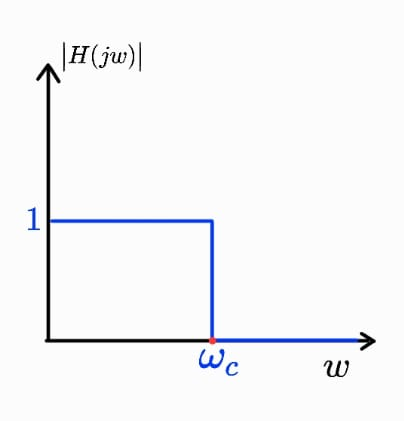
\includegraphics[width=\linewidth]{figuras/passa_baixa.png}
        \centering
        \\ \textbf{(a)}
    \end{minipage}
    \begin{minipage}[b]{0.32\linewidth}
        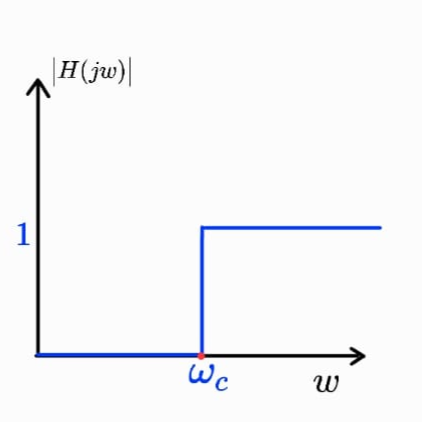
\includegraphics[width=\linewidth]{figuras/passa_altas.png}
        \centering
        \\ \textbf{(b)}
    \end{minipage}
    \begin{minipage}[b]{0.32\linewidth}     
        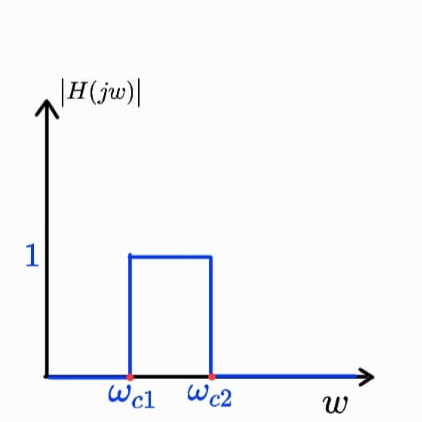
\includegraphics[width=\linewidth]{figuras/passa_faixa.png}
        \centering
        \\ \textbf{(c)}
    \end{minipage}
    \begin{minipage}[b]{0.32\linewidth}
        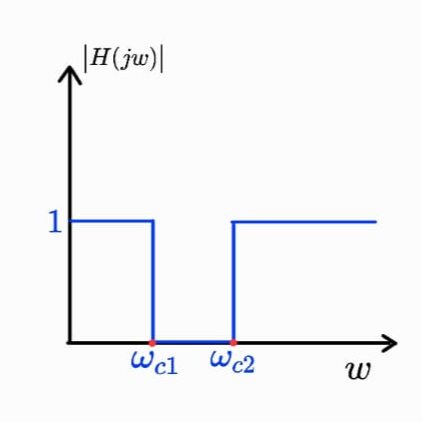
\includegraphics[width=\linewidth]{figuras/rejeita_faixa.png}
        \centering
        \\ \textbf{(d)}
    \end{minipage}
    \begin{minipage}[b]{0.32\linewidth}     
        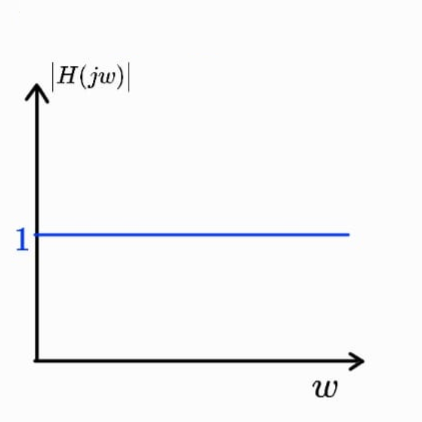
\includegraphics[width=\linewidth]{figuras/passa_tudo.png}
        \centering
        \\ \textbf{(e)}
    \end{minipage}
    \caption{Filtros básicos: (a) passa-baixa, (b) passa-alta, (c) passa-faixa, (d) rejeita-faixa e (e) passa-tudo.}
    \label{fig:filtros_basicos}
\end{figure}

A faixa de frequência em que o filtro apresenta pouca ou nenhuma atenuação é chamada de faixa de passagem, enquanto a faixa de frequência com atenuação significativa é chamada de faixa de rejeição. Uma das imperfeições dos filtros reais é que a transição entre a faixa de passagem e a faixa de rejeição não é abruta, mas sim graduação. A faixa que acontece essa transição é chamada de faixa de transição, tendo inicio na frequência $w_c$ e encerrando em uma frequência $w_s$, a qual é chamada de frequência de borda da faixa de rejeição. Outras imperfeições encontradas em filtros reais é que o filtro não atenua completamente ($\|H(w)\| > 0$) as frequências da faixa de rejeição e que ele apresenta atenuação $(\|H(w)\| < 1$) na faixa de passagem.

Diante das imperfeições dos filtros reais, é comum que além das especificações das frequências $w_c$ e $w_s$ também sejam especificações de projetos de filtros a atenuação máxima permitida na faixa de passagem $(A_{\text{max}})$ e atenuação mínima na faixa de rejeição $(A_{\text{min}})$. Essas especificações são ilustradas na figura~\ref{fig:filtros_reais} para os filtros passa-baixas, passa-altas, passa-faixa e rejeita-faixa. Note que as curvas em cada uma das faixas de frequência são apenas ilustrativas, pois a resposta em frequência de um filtro depende do projeto do mesmo. 

\begin{figure}[h!]
    \centering
    \begin{minipage}[b]{0.32\linewidth}
        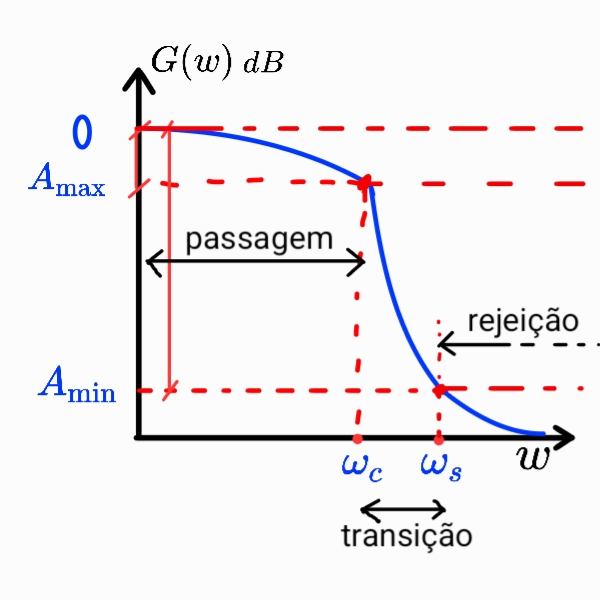
\includegraphics[width=\linewidth]{figuras/passa_baixas_real.png}
        \centering
        \\ \textbf{(a)}
    \end{minipage}
    \begin{minipage}[b]{0.32\linewidth}
        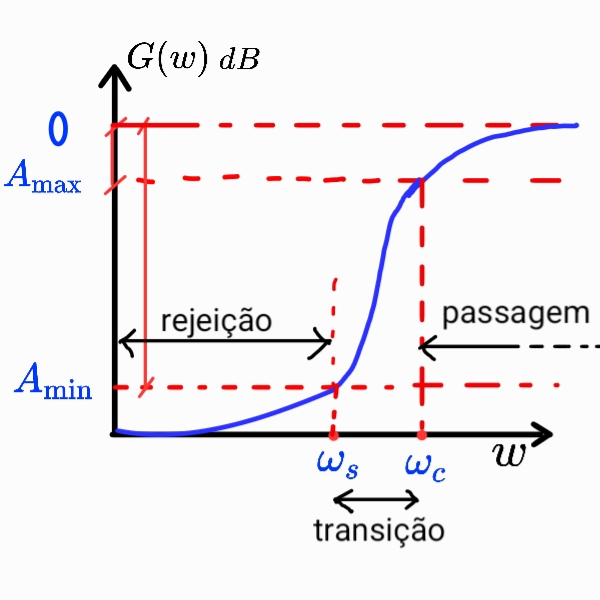
\includegraphics[width=\linewidth]{figuras/passa_altas_real.png}
        \centering
        \\ \textbf{(b)}
    \end{minipage}
    \\
    \begin{minipage}[b]{0.32\linewidth}     
        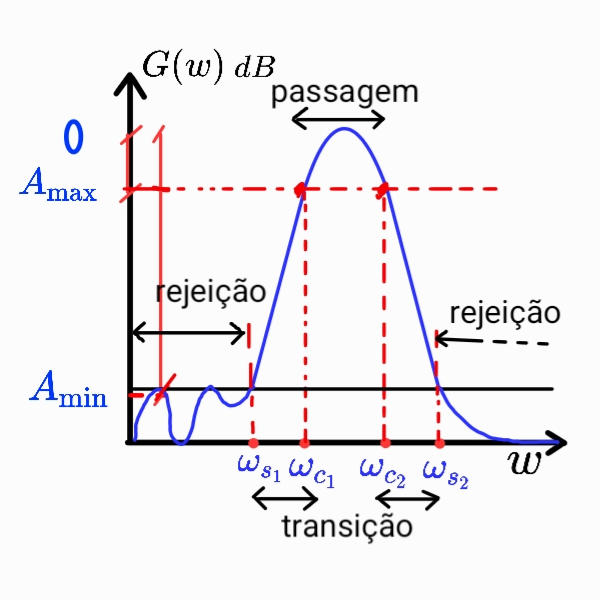
\includegraphics[width=\linewidth]{figuras/passa_faixa_real.png}
        \centering
        \\ \textbf{(c)}
    \end{minipage}
    \begin{minipage}[b]{0.32\linewidth}
        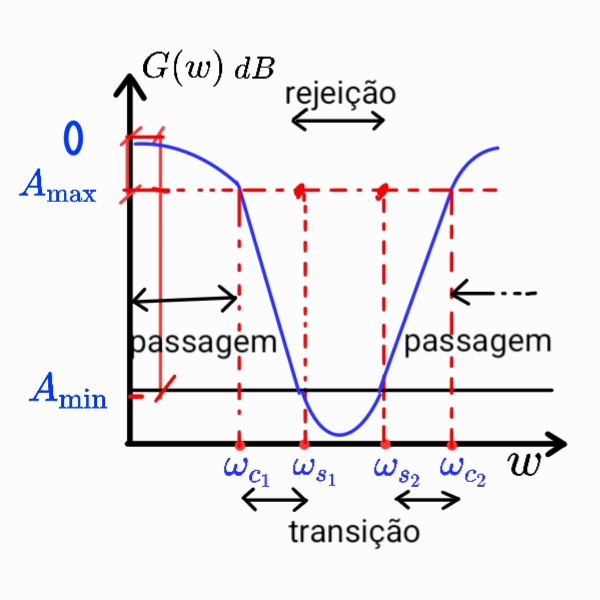
\includegraphics[width=\linewidth]{figuras/rejeita_faixa_real.png}
        \centering
        \\ \textbf{(d)}
    \end{minipage}
    \caption{Filtros básicos: (a) passa-baixa, (b) passa-alta, (c) passa-faixa, (d) rejeita-faixa.}
    \label{fig:filtros_reais}
\end{figure}

\section{Exemplos de filtros}

Na figura~\ref{fig:filtros_reais} estão apresentados exemplos circuitos de filtros passa-baixa, passa-alta e passa-faixa. As respostas em frequência desses circuitos são mostradas na figura~\ref{fig:LT_circuitos}.

\begin{figure}[h!]
    \centering
    \begin{minipage}[b]{0.32\linewidth}
        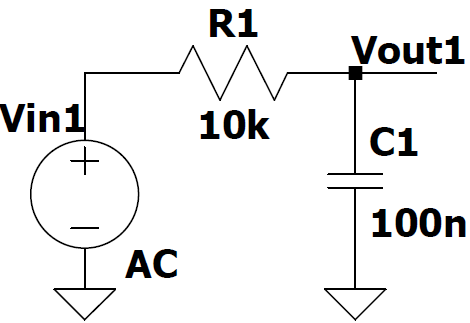
\includegraphics[width=\linewidth]{figuras/circuito_pb.png}
        \centering
        \\ \textbf{(a)}
    \end{minipage}
    \begin{minipage}[b]{0.32\linewidth}
        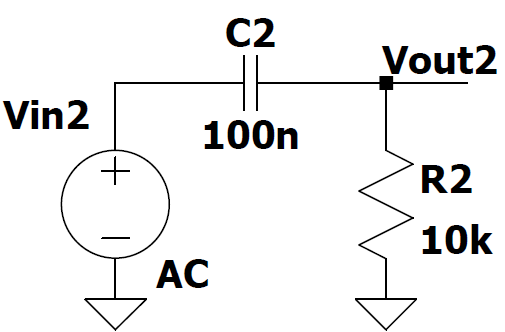
\includegraphics[width=\linewidth]{figuras/circuito_pa.png}
        \centering
        \\ \textbf{(b)}
    \end{minipage}
    \\
    \begin{minipage}[b]{0.49\linewidth}     
        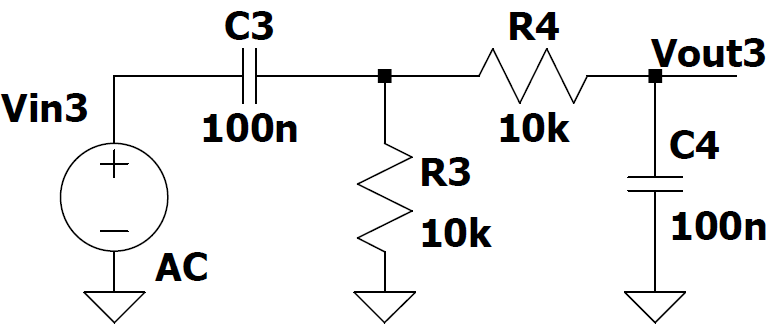
\includegraphics[width=\linewidth]{figuras/circuito_pf.png}
        \centering
        \\ \textbf{(c)}
    \end{minipage}
    %\begin{minipage}[b]{0.49\linewidth}
    %    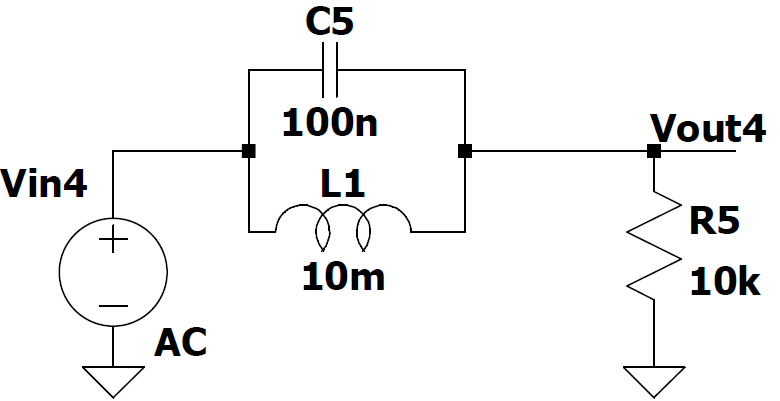
\includegraphics[width=\linewidth]{figuras/circuito_rf.png}
    %    \centering
    %    \\ \textbf{(d)}
    %\end{minipage}
    \caption{Exemplos de circuitos: (a) passa-baixa, (b) passa-alta, (c) passa-faixa.}
    \label{fig:filtros_reais}
\end{figure}

\begin{figure}[h!]
    \centering
    \begin{minipage}[b]{0.9\linewidth}
        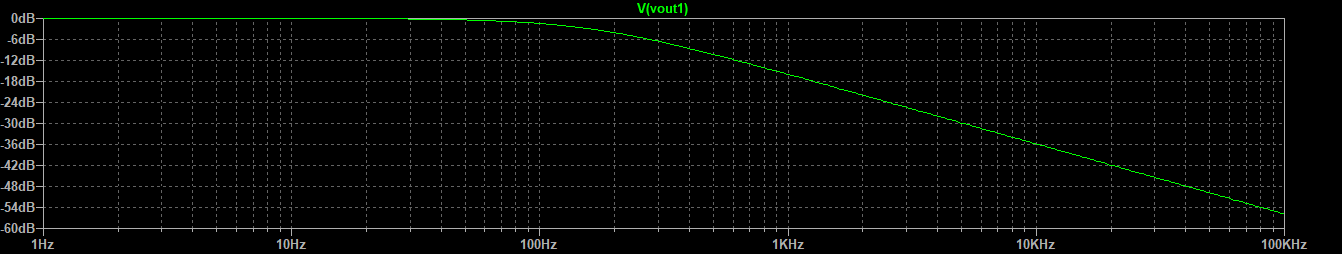
\includegraphics[width=\linewidth]{figuras/LT_pb.png}
        \centering
        \\ \textbf{(a)}
    \end{minipage}
    \begin{minipage}[b]{0.9\linewidth}
        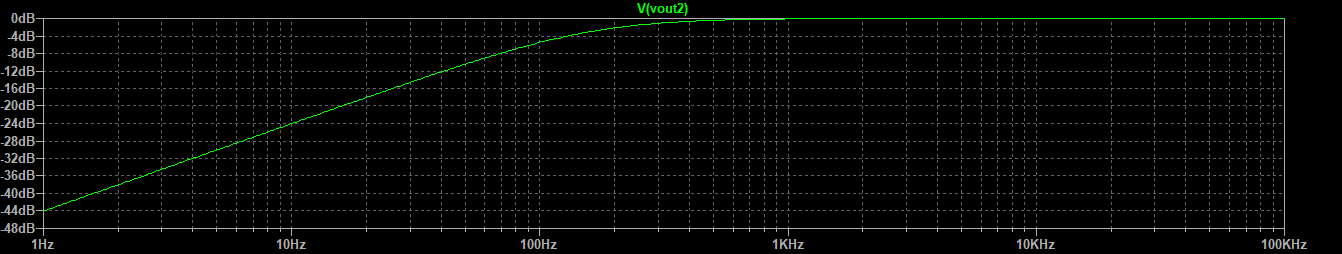
\includegraphics[width=\linewidth]{figuras/LT_pa.png}
        \centering
        \\ \textbf{(b)}
    \end{minipage}
    \begin{minipage}[b]{0.9\linewidth}     
        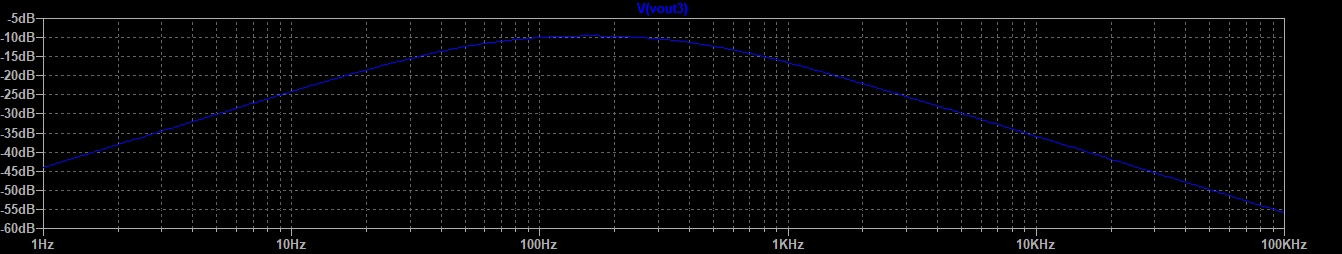
\includegraphics[width=\linewidth]{figuras/LT_pf.png}
        \centering
        \\ \textbf{(c)}
    \end{minipage}
    %\begin{minipage}[b]{0.9\linewidth}
    %    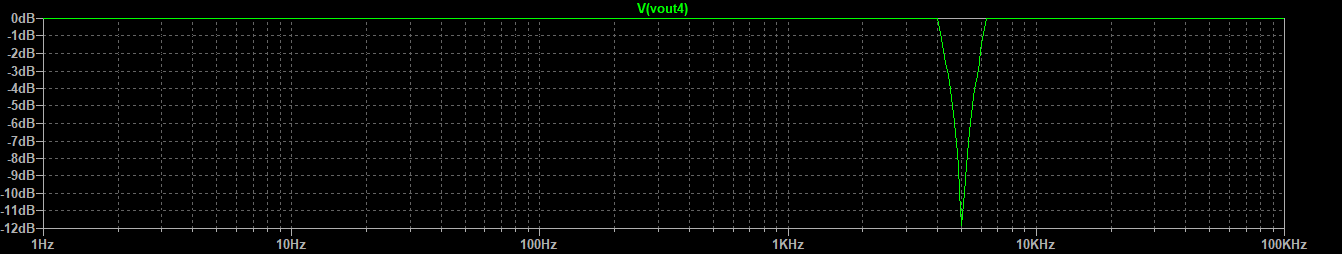
\includegraphics[width=\linewidth]{figuras/LT_rf.png}
    %    \centering
    %    \\ \textbf{(d)}
    %\end{minipage}
    \caption{Respostas dos filtros simuladas no LTspice: (a) passa-baixa, (b) passa-alta, (c) passa-faixa. Os arquivos de simulação estão disponíveis no \href{https://github.com/David1340/Apostila-Filtros-Ativos/tree/main/LTspice}{github}}
    \label{fig:LT_circuitos}
\end{figure}

  
\chapter{Problema da aproximação}
\label{chap: aproximacao}

O problema da aproximação é um conceito fundamental na teoria de controle e na análise de sistemas dinâmicos. Ele se refere à tarefa de encontrar uma representação matemática que se aproxime de maneira satisfatória o comportamento de um sistema real. Essa representação pode ser uma função, um modelo matemático ou uma estrutura de controle.

\section{Butterworth}

\section{Chebyshev}

\section{Elíptico}

A aproximação Elíptico também conhecida como aproximação de Cauer caracteriza-se por possui oscilações tanto na faixa de passagem quanto na faixa de rejeição. Em troca, ele obtém uma queda mais acentuada na faixa de transição, o que faz com que a aproximação de Cauer seja capaz de satisfazer as especificações de projeto de filtros com uma ordem menor do que seria obtidos se fossem usadas as aproximações de Butterworth e de Chebyshev. Na tabela \ref{tab:eliptico} são apresentados exemplos de funções de transferência de aproximações de filtros passa-baixas do tipo elíptico com $A_\text{max} = 0.5$ dB e ordem 2. 

\begin{table}[!h]
    \centering
    \renewcommand{\arraystretch}{2.0}  % aumenta o espaçamento entre as linhas
    \caption{Exemplos de funções de transferência de filtros elípticos para $A_\text{max}  = 0.5$ dB de ordem 2.}
    \begin{tabular}{|c|c|c|}
        \hline
        $\Omega_s$ & $1/H(s)$ & $A_\text{min}$ (dB) \\
        \hline 
        1.5 & $ \frac{0.38540(s^2 + 3.92705)}{s^2 + 1.03153s + 1.60319}$ & 8.3\\
        \hline
        2.0 & $\frac{0.20133(s^2 + 7.4641)}{s^2 +  1.24504s +  1.59179}$& 13.9 \\
        \hline
        3.0 & $\frac{0.083974(s^2 + 17.48528)}{s^2 +  1.35715s +  1.55532}$& 21.5 \\ 
        \hline       
    \end{tabular} 
    \label{tab:eliptico}
\end{table}

\section{Bessel}

As aproximações anteriores são focadas no ganho ou atenuação do filtro, porém em algumas aplicações como sistemas de transmissão digitais, a distorção de fase é um fator importante a ser considerado. A aproximação de Bessel é projetada para obter uma curva de fase tão plana quanto possível na faixa de passagem.

A aproximação de Bessel normalziada é dada por:

\begin{equation}
    H(s) = \frac{B_n(0)}{B_n(s)}
\end{equation}
em que $B_n(s)$ é enésimo termo do polinômio de Bessel o qual é definido pela forma recursiva:

\begin{equation}
    B_0(s) = 1 
\end{equation}

\begin{equation}
    B_1(s) = s + 1
\end{equation}

\begin{equation}
    B_n(s) = (2n -1)B_{n-1}(s) + s^2B_{n-2}(s)
\end{equation}
  
  
\chapter{Sensibilidade}
\label{chap: sensibilidade}

A sensibilidade de um circuito é a medida do grau de variação do funcionamento nominal dele devido as mudanças nos elementos que o compõem. Matematicamente, a sensibilidade de um parâmetro $p$ do circuito em relação ao valor de $x$ de um elemento do circuito é definida como
\begin{equation}
    S^p_{x} = \frac{\partial p}{\partial x} \cdot \frac{x}{p}   
    \label{eq:sensibilidade}
\end{equation}

Algumas relações úteis que podem ser derivadas a partir da equação \ref{eq:sensibilidade} são:

\begin{equation}
    S^c_{x} = 0 \quad \text{(c constante)},
\end{equation}

\begin{equation}
    S^{c x} _{x} = 1 \quad \text{(c constante)},
    \label{eq:constante2}
\end{equation}

\begin{equation}
    S^p_{x} = - S^{1/p}_{x},
    \label{eq:inversa}
\end{equation}

\begin{equation}
    S^{p_1 p_2}_{x} = S^{p_1}_{x} + S^{p_2}_{x},
\end{equation}

\begin{equation}
    S^{p_1 / p_2}_{x} = S^{p_1}_{x} - S^{p_2}_{x}
    \label{eq:divisao}
\end{equation}

\begin{equation}
    S^{p^n}_{x} =  nS^{p}_{x}
    \label{eq:potencia}
\end{equation}

\begin{equation}
    S^{p_1 + p_2}_{x} = \frac{p_1 S^{p_1}_{x} + p_2 S^{p_2}_{x}}{p_1 + p_2}
\end{equation}

\begin{equation}
    S^{cf(x)}_{x} = S^{f(x)}_x
    \label{eq:constante}
\end{equation}

\section{Exemplo de cálculo de sensibilidade}

Na figura~\ref{fig:MFB} é apresentado um exemplo de filtro passa-baixas de segunda ordem, cujos os parâmetros $H_0$, $\omega_0$  e $Q$ são dados por:

\begin{equation}
    H_0 = -\frac{R_5}{R_1},
    \label{eq:H0}
\end{equation}

\begin{equation}
    \omega_0^2 = \frac{1}{R_3 R_5 C_2 C_4},
    \label{eq:omega0}
\end{equation}

\begin{equation}
    W_0/Q = \frac{1}{C_2} (\frac{1}{R_1} + \frac{1}{R_3}  + \frac{1}{R_5} ).
    \label{eq:Q}
\end{equation}

\begin{figure}[h!]
    \centering
    \begin{minipage}[b]{0.9\linewidth}
        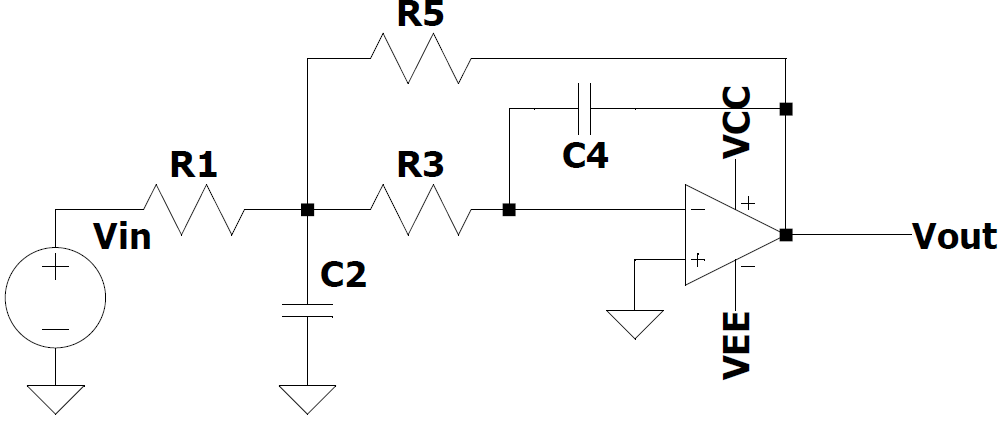
\includegraphics[width=\linewidth]{figuras/MFB.png}
        \centering
        \\ \textbf{(a)}
    \end{minipage}
    \caption{Oi}
    \label{fig:MFB}
\end{figure}

Com base na equação~\ref{eq:H0} e os as proprieades mostradas nas equações~\ref{eq:constante2} e~\ref{eq:inversa}, podemos calcular a sensibilidade de $H_0$ em relação a $R_1$ e $R_5$:	

\begin{equation}
    S^{H_0}_{R_1} = - S^{H_0}_{1/R_1} = -1,
\end{equation}

\begin{equation}
    S^{H_0}_{R_5} = 1.
\end{equation}

Com base na equação~\ref{eq:omega0} e as propriedades mostradas nas equações~\ref{eq:constante2},\ref{eq:inversa} e~\ref{eq:potencia}, podemos calcular a sensibilidade de $\omega_0$ em relação a $R_3$, $R_5$, $C_2$ e $C_4$:

\begin{equation}
    S^{\omega_0}_{R_3} = - S^{\omega_0}_{1/R_3} = -\frac{1}{2} S^{\omega_0}_{R^{-1/2}_3} = -\frac{1}{2},
\end{equation}

\begin{equation}
    S^{\omega_0}_{R_5} = S^{\omega_0}_{C_2} = S^{\omega_0}_{C_4} = S^{\omega_0}_{R_3} = - \frac{1}{2}
\end{equation}

Com base na equação~\ref{eq:Q} e as propriedades mostradas nas equações~\ref{eq:constante2},\ref{eq:inversa} e~\ref{eq:divisao}, podemos calcular a sensibilidade de $Q$ em relação a $R_1$, $R_3$, $R_5$ e $C_2$:

\begin{equation}
    S^{Q}_{x} = S^{\omega_0}_{x} - S^{\omega_0/Q}_{x} \quad \text{(x = $R_1$, $R_3$, $R_5$ e $C_2$)}
\end{equation}

\begin{equation}
    S^{\omega_0/Q}_{C_2} = -S^{\omega_0/Q}_{1/C_2} = -1
\end{equation}

\begin{equation}
    S^{\omega_0/Q}_{R_1} = -S^{\omega_0/Q}_{1/R_1} = -\frac{1/R_1}{1/R_1 + 1/R_3 + 1/R_5}
\end{equation}

\begin{equation}
    S^{\omega_0/Q}_{R_3} = -\frac{1/R_3}{1/R_1 + 1/R_3 + 1/R_5}
\end{equation}

\begin{equation}
    S^{\omega_0/Q}_{R_5} = -\frac{1/R_5}{1/R_1 + 1/R_3 + 1/R_5}
\end{equation}

  \backmatter
  \bibliographystyle{unsrt-br}
  \bibliography{main.bib}
  

\end{document}

